\subsubsection{MF1. Módulo de procesamiento}

\subsubsubsection{MF1.1. Procesamiento de la respuesta y cálculo de la acústica}

A partir de la respuesta al impulso de un recinto, se pueden derivar distintos parámetros acústicos, como los establecidos en la \href{https://www.iso.org/standard/36201.html}{ISO-3382}. Siendo que la respuesta al impulso la podemos obtener de mediciones físicas, de simulaciones del recinto, e incluso de bancos de datos con respuestas de múltiples recintos para fines de validación, fue necesario tener una metodología general que nos permitiera analizar datos de diferentes fuentes. \hfill\break
El programa de generación y medición de la acústica, tiene como salida una estructura con los datos de la respuesta al impulso y el tiempo de muestreo; para las simulaciones y los bancos de datos, las respuestas al impulso se guardan como un archivo de tipo \textit{wav}. Se iniciará con una línea de lectura de archivos de este tipo, que se desactivara en caso de usarse consecutivo al programa de generación y medición de la acústica. Dicho código también se encargara de combinar las señales en caso de leer archivos \textit{wav} con múltiples canales.
\begin{lstlisting}[frame=single,numbers=left, style=Matlab-editor, basicstyle=\tiny]
[temp_y,ImpulseResponse.fs] = audioread(['C:\Users\User\Desktop\RIR_Database\' ...
    '382908__uzbazur__little-basement-ir-impulse-response.wav']);
if size(temp_y,2) > 1
    ImpulseResponse.y = mean(temp_y,2);
end
\end{lstlisting}
De acuerdo con la norma ISO-3382, los parámetros acústicos que caracterizan un cuarto son:
\begin{itemize}
    \item $EDT$, tiempo de decaimiento temprano
    \item $T_{20}$ tiempo de reverberación referido a -20 Db
    \item $T_{30}$ tiempo de reverberación referido a -30 Db
    \item $C_{50}$ claridad a 50 ms
    \item $C_{80}$ claridad a 80 ms
    \item $D_{50}$ ratio de energía útil
    \item $G$ fuerza del sonido 
\end{itemize}
Todos los parámetros anteriores, deben calcularse en las frecuencias centrales de las bandas de frecuencia pertenecientes octavas de 125 Hz a 4000 Hz. Por esto, primero se deben pasar por filtros pasa-bandas, distribuidos a lo largo de las octavas.
Se paso la respuesta al impulso por 6 filtros, con frecuencias centrales y rangos como se muestra a continuación \href{https://www.doctorproaudio.com/content.php?2402-octaves-and-third-octaves#:~:text=As%20a%20reference%2C%20the%20central,exactly%20to%20double%20or%20half.}{Fuente}:
\begin{center}
    \begin{longtable}[!htb]{ |c|c|c| }
    \hline
    Frecuencia central & Limite inferior & Limite superior \\
    \hline
    125 Hz & 88.39 Hz & 176.8 Hz \\
    250 Hz & 176.8 Hz & 353,6 Hz \\
    500 Hz & 353.6 Hz & 707.1 Hz \\
    1000 Hz & 707.1 Hz & 1414 Hz \\
    2000 Hz & 1414 Hz & 2828 Hz \\
    4000 Hz & 2828 Hz & 5657 HZ \\
    \hline
    \caption{Rangos de frecuencias para filtros}
    \label{tab:Rangos De Frecuencias}
    \end{longtable} 
\end{center}
\begin{lstlisting}[frame=single,numbers=left, style=Matlab-editor, basicstyle=\tiny]
RIR = struct('General',ImpulseResponse); 
RIR.f125.y = bandpass(ImpulseResponse.y,[88.39 176.8],ImpulseResponse.fs);
RIR.f125.fs = ImpulseResponse.fs;
RIR.f250.y = bandpass(ImpulseResponse.y,[176.8 353.6],ImpulseResponse.fs);
RIR.f250.fs = ImpulseResponse.fs;
RIR.f500.y = bandpass(ImpulseResponse.y,[353.6 707.1],ImpulseResponse.fs);
RIR.f500.fs = ImpulseResponse.fs;
RIR.f1k.y = bandpass(ImpulseResponse.y,[707.1 1414],ImpulseResponse.fs);
RIR.f1k.fs = ImpulseResponse.fs;
RIR.f2k.y = bandpass(ImpulseResponse.y,[1414 2828],ImpulseResponse.fs);
RIR.f2k.fs = ImpulseResponse.fs;
RIR.f4k.y = bandpass(ImpulseResponse.y,[2828 5657],ImpulseResponse.fs);
RIR.f4k.fs = ImpulseResponse.fs;
\end{lstlisting}
Se pueden observar algunas la respuesta del recinto para ciertas frecuencias.
\begin{figure}[!htb]
    \centering
    \begin{subfigure}{0.3\textwidth}
        \centering
        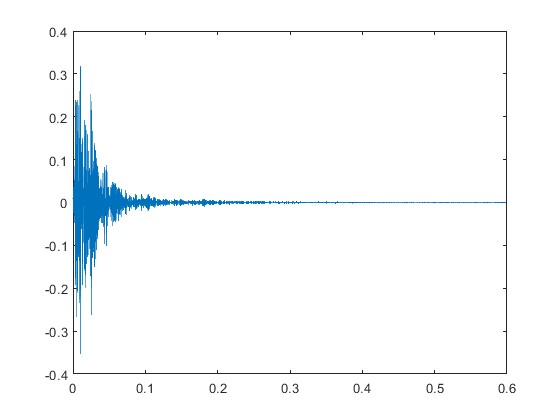
\includegraphics[width=\linewidth]{imagenes/RIR_500Hz_RIR_Measurement.jpg}
        \caption{\footnotesize Respuesta al impulso a 500 Hz}
        \label{fig:sub1}
    \end{subfigure}
    \hfill
    \begin{subfigure}{0.3\textwidth}
        \centering
        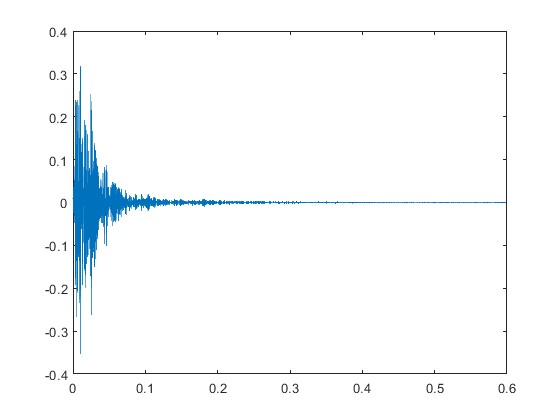
\includegraphics[width=\linewidth]{imagenes/RIR_1000Hz_RIR_Measurement.jpg}
        \caption{\footnotesize Respuesta al impulso a 1000 Hz}
        \label{fig:sub2}
    \end{subfigure}
    \hfill
    \begin{subfigure}{0.3\textwidth}
        \centering
        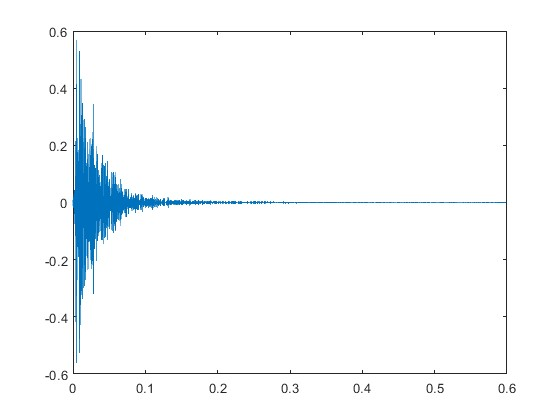
\includegraphics[width=\linewidth]{imagenes/RIR_2000Hz_RIR_Measurement.jpg}
        \caption{\footnotesize Respuesta al impulso a 2000 Hz}
        \label{fig:sub2}
    \end{subfigure}
    \caption{Respuesta al impulso para diferentes frecuencias}
\end{figure}
\FloatBarrier

A continuación podemos hacer el análisis de la respuesta al impulso en sus diferentes frecuencias, además de la general, lo que nos dará los parámetros acústicos actuales del recinto. Este proceso se hace mediante otro \textit{script} llamado \textbf{$RIR\_Analysis$}.\hfill\break
La función toma como primera entrada el método de empaquetado de la señal, se debe ingresar un 1 en caso de que se quiera analizar un archivo de tipo \textit{wav}, y cualquier otro numero en caso de que la señal ya venga empaquetada en una estructura con el tiempo de muestreo y la amplitud. A continuación se introduce la señal correspondiente, además de las dimensiones del cuarto en el que se grabo la respuesta al impulso y una variable booleana que indica al programa si debe mostrar la gráfica de decaimiento de la energía junto con los ajustes lineales y los parámetros.
La función retorna la respuesta al impulso cuadrada, la gráfica de decaimiento, el vector de tiempo correspondiente y una estructura con los parámetros acústicos.

\begin{lstlisting}[frame=single,numbers=left, style=Matlab-editor, basicstyle=\tiny]
function [RIRsq,DC,t,AcousticParams] = RIR_Analisys(method, input, room_dimensions,printFlag)
\end{lstlisting}
La gráfica del decaimiento se obtiene mediante la integral de Schroeder, la cual es una integración hacia atrás, que se hace desde un punto donde la señal ya solo contiene ruido de fondo. \href{https://www.roomeqwizard.com/help/help_en-GB/html/graph_filteredir.html}{Fuentes}
\begin{lstlisting}[frame=single,numbers=left, style=Matlab-editor, basicstyle=\tiny]
    RIRsq = y.^2;
    schroeder_cumsum = cumsum(flipud(RIRsq));
    schroeder_normalized = schroeder_cumsum / max(schroeder_cumsum);
    DC = flipud(10*log10(schroeder_normalized));
\end{lstlisting}
La gráfica se muestra en decibelios y va de 0 a $-\infty$. \\
La curva de decaimiento de la energía nos permite ver el decaimiento exponencial del sonido como un decaimiento lineal, y así, poder ajustar rectas que se apeguen mas al decaimiento de la señal sin verse interferida por el ruido de fondo. Adicionalmente, podemos usar esta curva para calcular los otros parámetros acústicos como $D_{50}$ o $C_{50}$.\hfill\break
\begin{figure}[!htb]
    \centering
    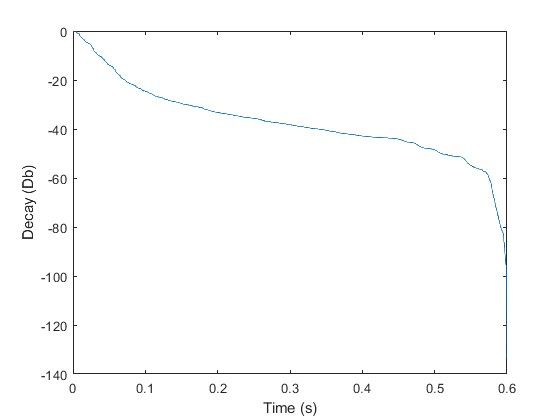
\includegraphics[width=\linewidth]{imagenes/DecayCurve_RIR_Analysis.jpg}
    \caption{\footnotesize Curva de decaimiento}
    \label{fig:DecayCurve}
\end{figure}
\FloatBarrier
El comportamiento de la curva deja de ser lineal cuando la señal comienza a verse afectada por el ruido de fondo. Idealmente, el ruido de fondo debería presentarse como un valle horizontal, y la señal con un decaimiento lo mas recto posible, hasta curvarse al final para convertirse en el valle del ruido de fondo. \hfill\break
El análisis de esta curva revela la importancia de tener una excitación lo bastante fuerte como para superar al ruido de fondo y ver el decaimiento de la curva por mas tiempo antes de comenzar a perder información. Es por esto también que, a pesar de que el tiempo de reverberación esta referido a -60 Db, no suele medirse el decaimiento de esta manera, si no que se recurre a medir un decaimiento de -20 Db o -30 Db y se hace una extrapolación hasta los -60 Db. La norma ISO-3382 recomienda comenzar a medir el decaimiento hasta los -5 Db, para evitar interferencias de armónicos y entonces disminuir 20 o 30 Db. Intentar observar el decaimiento hasta -65 Db, implica que para un ruido de fondo de unos 30 Db, requeriríamos excitar el cuarto con una señal de al menos 95 Db, lo cual escapa de las posibilidades dentro de un recinto relativamente pequeño.\hfill\break
Posteriormente, se ajustan rectas tomando en cuenta los intervalos de -20 Db, -30 Db y del EDT.
\begin{lstlisting}[frame=single,numbers=left, style=Matlab-editor, basicstyle=\tiny]
    [~, EDT_Idx1] = min(abs(LF_EDT+10));
    [~, EDT_Idx2] = min(abs(LF_EDT));
    T60delEDT = 6*(t(EDT_Idx1)-t(EDT_Idx2));
    
    [~, EDT_Idx1] = min(abs(LF_T20+20));
    [~, EDT_Idx2] = min(abs(LF_T20));
    T60delT20 = 3*(t(EDT_Idx1)-t(EDT_Idx2));
    
    [~, EDT_Idx1] = min(abs(LF_T30+30));
    [~, EDT_Idx2] = min(abs(LF_T30));
    T60delT30 = 2*(t(EDT_Idx1)-t(EDT_Idx2));
\end{lstlisting}
La relación de energía útil ($D$) se define como la relación entre la energía total y la energía de la señal con arribo temprano. Se utilizan $D_{50}$ y $D_{80}$ para definir este parámetro usando 50 y 80 ms respectivamente como el limite para el arribo temprano. Cabe resaltar que este tiempo se toma a partir del momento que llega la señal directa (en linea recta de la fuente al receptor).
\begin{lstlisting}[frame=single,numbers=left, style=Matlab-editor, basicstyle=\tiny]
    [~,maxIdx] = max(RIRsq);
    RIRsq_trunc = RIRsq(maxIdx:end);
    Energy0_50 = trapz(RIRsq_trunc(1:round(0.05*fs)));
    Energy0_80 = trapz(RIRsq_trunc(1:round(0.08*fs)));
    Energy0_end = trapz(RIRsq_trunc(1:end));
    
    D50 = Energy0_50/Energy0_end;
    D80 = Energy0_80/Energy0_end;
\end{lstlisting}
Los índices de claridad $C_{50}$ y $C_{80}$ siguen la misma definición que el índice $D$, pero, en lugar de representar un ratio o porcentaje, estos se presentan en Db como escala logarítmica. El índice $C_{50}$ se puede entender como la claridad del habla y $C_{80}$ como la claridad de la musica. Ambos se pueden calcular a partir del índice $D$ como:
$$C_{50/80} = 10 log \left( \frac{D_{50/80}}{1-D_{50/80}} \right)$$

\begin{lstlisting}[frame=single,numbers=left, style=Matlab-editor, basicstyle=\tiny]
    C50 = 10*log(D50/(1-D50));
    C80 = 10*log(D80/(1-D80));
\end{lstlisting}

Por ultimo, la fuerza del sonido $G$ se define como la relación entre el nivel de presión del sonido en el recinto y el nivel de presión del mismo sonido en un campo libre, es decir, sin reflexiones, únicamente el sonido directo. \hfill\break
La medición de este parámetro es un poco mas complicada, ya que se requiere aislar de todas las reflexiones, al pico en la amplitud producido por el sonido directo. Por esto, se decidió hacer una estimación validada por \cite{Rossing2007}, que relaciona la fuerza del sonido con el tiempo de reverberación en un recinto y sus dimensiones.
$$G = 10 log_{10}\left(\frac{RT_{60}}{V}\right)$$

El ultimo análisis que se hace a la respuesta al impulso es respecto a los modos de vibración. Un recinto con paredes ortogonales, presenta distancias entre paredes que es un múltiplo de la longitud de onda de distintas frecuencias. Lo anterior ocasiona que las ondas oscilen entre paredes como si estuvieran ancladas a las paredes. Cuando el sonido es persistente o el tiempo de reverberación alto, un oyente puede encontrar que existen zonas del cuarto donde el sonido es muy fuerte y otras donde el sonido es muy bajo y se puede medir el cambio en el volumen si se desplaza por el recinto. \\
Los modos de vibración pueden ser axiales, tangenciales y oblicuos, dependiendo del numero de superficies en las que rebota. Los modos de vibración axiales suelen ser los mas significativos y por suerte, son los mas fáciles de predecir. \\
Podemos calcular los modos de vibración calculando las frecuencias en donde las dimensiones del cuarto son múltiplos de sus respectivas longitudes de onda. El programa cuenta con un \textit{script} externo llamado \textbf{CalcRoomModes} que realiza esta operación. El programa retorna los primeros n modos axiales de vibración.
\begin{lstlisting}[frame=single,numbers=left, style=Matlab-editor, basicstyle=\tiny]
    c = 343; % m/s
    f_length = c/room_dim(1);
    f_width = c/room_dim(2);
    f_depth = c/room_dim(3);
    modes_length = zeros(1,num_modes);
    modes_width = zeros(1,num_modes);
    modes_depth = zeros(1,num_modes);

    for i = 1:num_modes
        modes_length(i) = f_length*(0.5*i); 
        modes_width(i) = f_width*(0.5*i);
        modes_depth(i) = f_depth*(0.5*i);
    end
\end{lstlisting}
Adicionalmente, el programa se encarga de calcular la frecuencia de Schroeder, la cual nos indica la frecuencia a la que el sonido dentro de un recinto deja de estar dominado por los modos de vibración y pasa a comportarse como un campo difuso. Se calcula con la siguiente formula:
$$f_s = 2000\sqrt{\frac{RT_{60}}{V}}$$
El calculo de este parámetro es importante, debido a que el resto de parámetros acústicos solo son validos si el sonido presente en el recinto se comporta mayormente como un campo difuso. Como se ve en la formula, la variable libre de la que depende esta frecuencia es el tiempo de reverberación; esto nos ayudara a introducir cotas para el tiempo de reverberación que nos asegure no tener modos de vibración significativos durante la reproducción de musica en el estudio.
La ecuación de Sabine (cita) relaciona el tiempo de reverberación con la absorción de las superficies del cuarto y su geometría. 
\begin{displaymath}
    RT_{60} = \frac{0.161 V}{S \alpha}
\end{displaymath}\
Podemos utilizar esta ecuación para tener una relación entre el tiempo de reverberación del cuarto y la superficie de absorción. Debido a que conocemos las absorciones tanto de los paneles como de las paredes, eso deja a la superficie como parámetro libre. Entonces, el control acústico consistirá en encontrar la cantidad de absorción especifica para alcanzar un tiempo de reverberación deseado, y con ella, obtener la cantidad de superficie de paneles acústicos que debemos añadir en el cuarto para alcanzar dicho tiempo de reverberación.
\begin{lstlisting}[frame=single,numbers=left, style=Matlab-editor, basicstyle=\tiny]
    V = prod(room_dim);
    Current_abs = 0.161*V/AcousticParams.General.T60delT20;
    DesiredT60 = 0.27
    Needed_abs = 0.161*V/DesiredT60;
    Offset_abs = Needed_abs-Current_abs;
    MaterialAbs.Abs_Panels = 0.8;
    MaterialAbs.Wall = 0.02;
    Surface = Offset_abs/(MaterialAbs.Abs_Panels-MaterialAbs.Wall)  
\end{lstlisting}

%--------------------------------------------------------------------
\paragraph{RayTracingImpulseResponse}\hfill \break
En este programa se simula la respuesta al impulso en una sala con el objetivo de modelar las propiedades reverberantes de un espacio sin tener que realizar mediciones acústicas. La metodología usada presente en \href{http://publications.rwth-aachen.de/record/50580/files/3875.pdf}{Real-Time Auralization}, consiste en tratar el sonido como rayos que viajan en un recinto, los cuales se emiten de manera aleatoria y uniforme, y chocan contra diferentes superficies, perdiendo energía en el proceso. Además, cuando los rayos chocan con una superficie esta refleja los rayos de manera difusa, por lo que una parte de la energía termina en el receptor. La simulación consiste en seguir el camino de los rayos para observar como pierden energía y calcular cuanta energía llega al receptor en cada reflexión, esto para construir un histograma dependiente de la frecuencia y después, obtener la respuesta al impulso pesando un proceso aleatorio de Poisson con el histograma. \\
El programa esta basado en una implementación derivada de \href{https://www.mathworks.com/help/audio/ug/room-impulse-response-simulation-with-stochastic-ray-tracing.html}{\textit{Room Impulse Response Simulation with Stochastic Ray Tracing}}, la cual no nos permite tener caracteristicas localizadas, sino que las toma uniformes en toda la pared, lo cual entre en conflicto con la colocación de paneles acústicos. \\
Para empezar se colocan las dimensiones de la sala, para posteriormente colocar las posiciones del emisor y del receptor y colocar el radio del micrófono, el cual en este caso es de 8.75cm.\\
\begin{figure}[!htb]
    \centering
    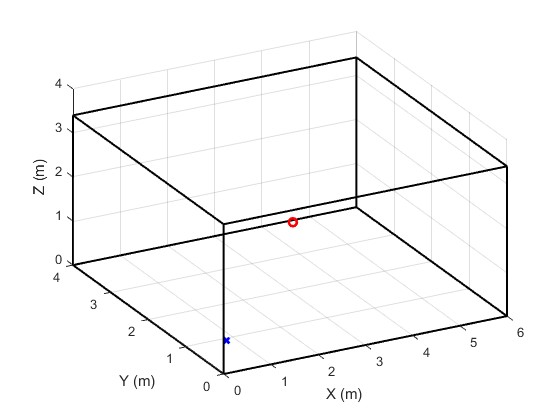
\includegraphics[width=\linewidth]{imagenes/plotRoom.jpg}
    \caption{\footnotesize Geometría del cuarto simulado y posiciones del emisor y receptor}
    \label{fig:plotRoom}
\end{figure}
\FloatBarrier
En la siguiente sección se generan los rayos, los cuales son emanados de la fuente en direcciones aleatorias. Para generar los rayos se utiliza la función RandSampleSphere, dichos rayos son una matriz N por 3 y cada fila de rayos mantiene la dirección del vector de rayos tridimensional.\\
Posteriormente en el código se definen los coeficientes de reflexión y dispersión. Un rayo de sonido se refleja cuando incide sobre una superficie. La reflexión es una combinación de un componente especular y un componente difuso. El coeficiente de absorción es una medida de cuánto sonido se absorbe (en lugar de reflejarse) al golpear una superficie, mientras que el coeficiente de difusión indica que tan especular o difusa es la reflexión.\\
Debido a que los parámetros acústicos se calculan para diferentes bandas de frecuencia, se tiene que hacer un análisis en diferentes frecuencias, dadas por FVect.
\begin{lstlisting}[frame=single,numbers=left, style=Matlab-editor, basicstyle=\tiny]
clear; close all; clc;

%% SetUp
SetUpStruct.room = [10 8 4];
SetUpStruct.src_pos = [2 2 2];
SetUpStruct.mic_pos = [5 5 1.8];
SetUpStruct.mic_radius = 0.0875;
impResTime = 10;

plotRoom(SetUpStruct.room,SetUpStruct.mic_pos,SetUpStruct.src_pos,1)

%% Generate Rays
N = 5000;
rng(0)
rays = RandSampleSphere(N);

%% Reflections and Scattering Coefficients
FVect = [125 250 500 1000 2000 4000];

abs_coeffs = [];
abs_coeffs(:,1) = [0.02,0.02,0.03,0.03,0.04,0.05,0.05]; %Concrete
abs_coeffs(:,2) = [0.70,0.45,0.65,0.60,0.75,0.65,0.65]; %AbsPanels
abs_coeffs(:,3) = [0.14,0.10,0.06,0.08,0.10,0.10,0.10]; %Door

scatt_coeffs = [];
scatt_coeffs(:,1) = [0.30,0.50,0.60,0.60,0.70,0.70,0.70];
scatt_coeffs(:,2) = [0.30,0.50,0.60,0.60,0.70,0.70,0.70];
scatt_coeffs(:,3) =  [0.30,0.50,0.60,0.60,0.70,0.70,0.70];
\end{lstlisting}
A continuación se hace la modificación al programa, creando un mapa de cada una de las paredes, que contiene valores diferentes de absorción y difusión para cada centímetro cuadrado de la pared. 
\begin{lstlisting}[frame=single,numbers=left, style=Matlab-editor, basicstyle=\tiny]
abs_map = {};
abs_map{1} = zeros(round(room_dim(2)*100),round(room_dim(3)*100),num_FBands);
abs_map{2} = zeros(round(room_dim(2)*100),round(room_dim(3)*100),num_FBands);
abs_map{3} = zeros(round(room_dim(1)*100),round(room_dim(3)*100),num_FBands);
abs_map{4} = zeros(round(room_dim(1)*100),round(room_dim(3)*100),num_FBands);
abs_map{5} = zeros(round(room_dim(1)*100),round(room_dim(2)*100),num_FBands);
abs_map{6} = zeros(round(room_dim(1)*100),round(room_dim(2)*100),num_FBands);

scatt_map = {};
scatt_map{1} = zeros(round(room_dim(2)*100),round(room_dim(3)*100),num_FBands);
scatt_map{2} = zeros(round(room_dim(2)*100),round(room_dim(3)*100),num_FBands);
scatt_map{3} = zeros(round(room_dim(1)*100),round(room_dim(3)*100),num_FBands);
scatt_map{4} = zeros(round(room_dim(1)*100),round(room_dim(3)*100),num_FBands);
scatt_map{5} = zeros(round(room_dim(1)*100),round(room_dim(2)*100),num_FBands);
scatt_map{6} = zeros(round(room_dim(1)*100),round(room_dim(2)*100),num_FBands);
\end{lstlisting}
A continuación, la función \textit{updateAbsScattCoefs} nos ayuda a actualizar los mapas de absorción y difusión, colocando los valores de absorción y difusión correspondientes a cada banda de frecuencia, en las índices del mapa correspondientes a sus posiciones en la pared.
\begin{lstlisting}[frame=single,numbers=left, style=Matlab-editor, basicstyle=\tiny]
[abs_map, scatt_map] = updateAbsScattCoeffs(abs_map,scatt_map,1,abs_coeffs(:,1),...
    scatt_coeffs(:,1),[0,0],[room_dim(2),room_dim(3)]); %SmallWall
[abs_map, scatt_map] = updateAbsScattCoeffs(abs_map,scatt_map,2,abs_coeffs(:,1),...
    scatt_coeffs(:,1),[0,0],[room_dim(2),room_dim(3)]); %OpSmallWall
[abs_map, scatt_map] = updateAbsScattCoeffs(abs_map,scatt_map,3,abs_coeffs(:,1),...
    scatt_coeffs(:,1),[0,0],[room_dim(1),room_dim(3)]); %LargeWall
[abs_map, scatt_map] = updateAbsScattCoeffs(abs_map,scatt_map,4,abs_coeffs(:,1),...
    scatt_coeffs(:,1),[0,0],[room_dim(1),room_dim(3)]); %OpLargeWall
[abs_map, scatt_map] = updateAbsScattCoeffs(abs_map,scatt_map,5,abs_coeffs(:,1),...
    scatt_coeffs(:,1),[0,0],[room_dim(1),room_dim(2)]); %Floor
[abs_map, scatt_map] = updateAbsScattCoeffs(abs_map,scatt_map,6,abs_coeffs(:,1),...
    scatt_coeffs(:,1),[0,0],[room_dim(1),room_dim(2)]); %Ceiling
\end{lstlisting}
Como los mapas están vacíos al crearse, primero se definen todas las paredes del cuarto con los respectivos coeficientes de absorción y difusión, y posteriormente ya se pueden actualizar ciertas zonas, con los coeficientes correspondientes a los paneles. \\
El mapa de reflexiones se obtiene a partir del mapa de absorción siguiendo la siguiente \href{https://www.researchgate.net/publication/276288771_Scattering_in_Room_Acoustics_and_Related_Activities_in_ISO_and_AES}{formula}
\begin{displaymath}
    Ref = \sqrt{1-Abs}
\end{displaymath}
\begin{lstlisting}[frame=single,numbers=left, style=Matlab-editor, basicstyle=\tiny]
ref_map = cell(1,num_FBands);
for i = 1:numel(abs_map)
    ref_map{i} = sqrt(1-abs_map{i});
end
\end{lstlisting}
Se definen tambien los parametros del histograma.
\begin{lstlisting}[frame=single,numbers=left, style=Matlab-editor, basicstyle=\tiny]
histTimeStep = 0.0010;
nTBins = round(impResTime/histTimeStep);
nFBins = length(FVect);
TFHist = zeros(nTBins,nFBins);
\end{lstlisting}
El proceso de \textit{Ray-Tracing} comienza tomando un rayo dentro de una banda de frecuencia, tomando su posición, dirección, el tiempo del rayo y su energía, y posteriormente, calcular en donde va a colisionar. Esto se hace observando los signos de la dirección del rayo, los cuales nos dice con cual, de entre dos paredes paralelas, va a colisionar el rayo. A continuación, se calcula el desplazamiento necesario para llegar a la coordenada constante de una pared y resaltando que chocara con la pared para la que necesite el menor desplazamiento. Este calculo se hace dentro de la funcion \textit{GetImpactWall}
\begin{lstlisting}[frame=single,numbers=left, style=Matlab-editor, basicstyle=\tiny]
function [surfaceofimpact,displacement] = getImpactWall(ray_xyz,ray_dxyz,roomDims)
% GETIMPACTWALL Determine which wall the ray encounters
surfaceofimpact = -1;
displacement = 1000;
%  Compute time to intersection with x-surfaces
if (ray_dxyz(1) < 0)
    displacement = -ray_xyz(1) / ray_dxyz(1);
    if displacement==0
        displacement=1000;
    end
    surfaceofimpact = 1; %"SmallWall"
elseif (ray_dxyz(1) > 0)
    displacement = (roomDims(1) - ray_xyz(1)) / ray_dxyz(1);
    if displacement==0
        displacement=1000;c
    end
    surfaceofimpact = 2; %"OpSmallWall"
end
% Compute time to intersection with y-surfaces
if ray_dxyz(2)<0
    t = -ray_xyz(2) / ray_dxyz(2);
    if (t<displacement) && t>0
        surfaceofimpact = 3; %"LargeWall";
        displacement = t;
    end
elseif ray_dxyz(2)>0
    t = (roomDims(2) - ray_xyz(2)) / ray_dxyz(2);
    if (t<displacement) && t>0
        surfaceofimpact =  4; %"OpLargeWall";
        displacement = t;
    end
end
% Compute time to intersection with z-surfaces
if ray_dxyz(3)<0
    t = -ray_xyz(3) / ray_dxyz(3);
    if (t<displacement) && t>0
        surfaceofimpact = 5; %"Floor";
        displacement = t;
    end
elseif ray_dxyz(3)>0
    t = (roomDims(3) - ray_xyz(3)) / ray_dxyz(3);
    if (t<displacement) && t>0
        surfaceofimpact = 6; %"Ceiling";
        displacement = t;
    end
end

displacement = displacement * ray_dxyz;

end
\end{lstlisting}
El desplazamiento y la pared de impacto, nos permite obtener las coordenadas en las que choca el rayo y así, consultar nuestro mapa de reflexión y difusión, para calcular el decaimiento de la energía con base en la reflexión y una nueva dirección para el rayo, la cual es combinación de la reflexión especular y la difusa. \\
Adicionalmente, se usa la difusión en ese punto, para calcular que cantidad de la energía restante del rayo va a capturar el receptor, la cual disminuye conforme mas se aleja del vector normal de la pared. \\
Este proceso se repite para la nueva posición, dirección, tiempo y energía del rayo; hasta que se supere el tiempo de simulación o la energía del rayo disminuya hasta ser despreciable.
\begin{lstlisting}[frame=single,numbers=left, style=Matlab-editor, basicstyle=\tiny]
for iBand = 1:nFBins
    fprintf("Calculating rays for band %d\n",iBand)
    % Perform ray tracing independently for each frequency band.
    for iRay = 1:size(rays,1)
        % Select ray direction
        ray = rays(iRay,:);
        % All rays start at the source/transmitter
        ray_xyz = source_pos;
        % Set initial ray direction. This direction changes as the ray is
        % reflected off surfaces.
        ray_dxyz = ray;
        % Initialize ray travel time. Ray tracing is terminated when the
        % travel time exceeds the impulse response length.
        ray_time = 0;
        % Initialize the ray energy to a normalized value of 1.     Energy
        % decreases when the ray hits a surface.
        ray_energy = 1;

        while (ray_time <= impResTime)

            % Determine the surface that the ray encounters
            [surfaceofimpact,displacement] = getImpactWall(ray_xyz,...
                                             ray_dxyz,room_dim);
            
            % Determine the distance traveled by the ray
            distance = sqrt(sum(displacement.^2));

            % Determine the coordinates of the impact point
            impactCoord = ray_xyz+displacement;

            if surfaceofimpact > 4
                pointOfImpact = [impactCoord(1),impactCoord(2)];
            elseif surfaceofimpact < 3
                pointOfImpact = [impactCoord(2),impactCoord(3)];
            else
                pointOfImpact = [impactCoord(1),impactCoord(3)];
            end

            % Update ray location/source
            ray_xyz = impactCoord;

            % Update cumulative ray travel time
            c = 343; % speed of light (m/s)
            ray_time = ray_time+distance/c;

            % Apply surface reflection to ray's energy
            % This is the amount of energy that is not lost through
            % absorption.

            ReflectionAtPoint = ref_map{surfaceofimpact}(ceil(100*pointOfImpact(1)),ceil(100*pointOfImpact(2)),iBand);
            ray_energy = ray_energy*ReflectionAtPoint;

            % Apply diffuse reflection to ray energy
            % This is the fraction of energy used to determine what is
            % detected at the receiver
            DifussionAtPoint = scatt_map{surfaceofimpact}(ceil(100*pointOfImpact(1)),ceil(100*pointOfImpact(2)),iBand);
            rayrecv_energy = ray_energy*DifussionAtPoint;

            % Determine impact point-to-receiver direction.
            rayrecvvector = mic_pos-impactCoord;

            % Determine the ray's time of arrival at receiver.
            distance = sqrt(sum(rayrecvvector.*rayrecvvector));
            recv_timeofarrival = ray_time+distance/c;

            if recv_timeofarrival>impResTime
                break
            end

            if ray_energy < 0.000001
                break
            end

            % Determine amount of diffuse energy that reaches the receiver.
            % See (5.20) in [2].

            % Compute received energy
            N = getWallNormalVector(surfaceofimpact);
            cosTheta = sum(rayrecvvector.*N)/(sqrt(sum(rayrecvvector.^2)));
            cosAlpha = sqrt(sum(rayrecvvector.^2)-mic_radius^2)/sum(rayrecvvector.^2);
            E = (1-cosAlpha)*2*cosTheta*rayrecv_energy;

            % Update energy histogram
            tbin = floor(recv_timeofarrival/histTimeStep + 0.5);
            TFHist(tbin,iBand) = TFHist(tbin,iBand) + E;

            % Compute a new direction for the ray.
            % Pick a random direction that is in the hemisphere of the
            % normal to the impact surface.
            d = rand(1,3);
            d = d/norm(d);
            if sum(d.*N)<0
                d = -d;
            end

            % Derive the specular reflection with respect to the incident
            % wall
            ref = ray_dxyz-2*(sum(ray_dxyz.*N))*N;

            % Combine the specular and random components
            d = d/norm(d);
            ref = ref/norm(ref);
            ray_dxyz = DifussionAtPoint*d+(1-DifussionAtPoint)*ref;
            ray_dxyz = ray_dxyz/norm(ray_dxyz);
        end
    end
end
\end{lstlisting}
Este proceso nos deja con un histograma dependiente de la frecuencia, el cual representa la envoltura de la respuesta al impulso.
\begin{figure}[!htb]
    \centering
    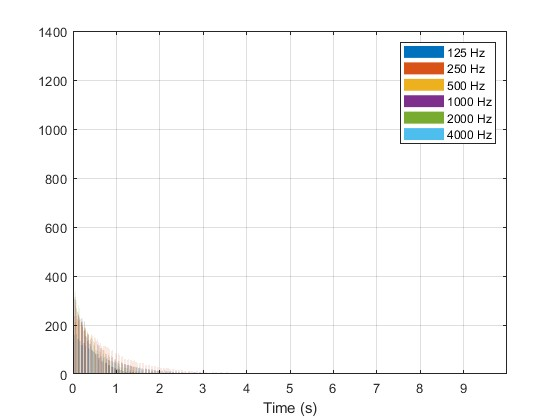
\includegraphics[width=\linewidth]{imagenes/Histogram.jpg}
    \caption{\footnotesize Histograma dependiente de la frecuencia}
    \label{fig:Histograma}
\end{figure}
\FloatBarrier
Para la construcción de la respuesta al impulso, es necesario modelar la estructura detallada a partir del histograma. Esto se puede hacer mediante ruido aleatorio con una distribución de Poisson, y se construye tomando la reflexión de un rayo como evento.\\
Es importante pasar el proceso aleatorio de Poisson por filtros pasa bandas que empaten con las frecuencias del histograma, para asi, poder multiplicarlos. 
\begin{figure}[!htb]
    \centering
    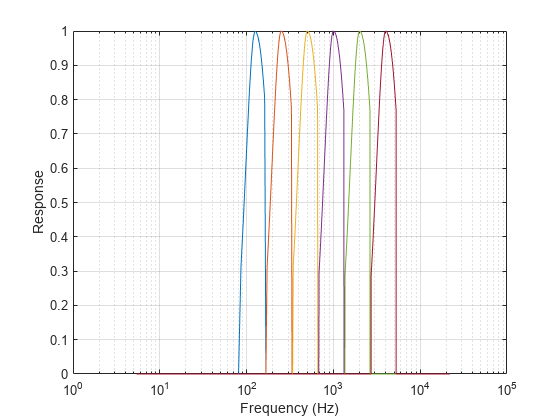
\includegraphics[width=\linewidth]{imagenes/BandPassFilters.png}
    \caption{\footnotesize Filtros pasa-bandas para el proceso de Poisson}
    \label{fig:PoissonFilters}
\end{figure}
\FloatBarrier
\begin{lstlisting}[frame=single,numbers=left, style=Matlab-editor, basicstyle=\tiny]
fs = 44100;
V = prod(room_dim);
t0 = ((2*V*log(2))/(4*pi*c^3))^(1/3); % eq 5.45 in [2]
poissonProcess = [];
timeValues = [];
t = t0;
while (t<impResTime)
    timeValues = [timeValues t]; %#ok
    % Determine polarity.
    if (round(t*fs)-t*fs) < 0 
        poissonProcess = [poissonProcess 1]; %#ok
    else
        poissonProcess = [poissonProcess -1];%#ok
    end
    % Determine the mean event occurence (eq 5.44 in [2])
    mu = min(1e4,4*pi*c^3*t^2/V); 
    % Determine the interval size (eq. 5.44 in [2])
    deltaTA = (1/mu)*log(1/rand); % eq. 5.43 in [2])
    t = t+deltaTA;
end
randSeq = zeros(ceil(impResTime*fs),1);
for index=1:length(timeValues)
    randSeq(round(timeValues(index)*fs)) = poissonProcess(index);
end
flow = [115 225 450 900 1800 3600 7200];
fhigh = [135 275 550 1100 2200 4400 8800];
NFFT = 8192;
win = hann(882,"symmetric");
sfft = dsp.STFT(Window = win,OverlapLength=441,FFTLength=NFFT,FrequencyRange="onesided");
isfft = dsp.ISTFT(Window=win,OverlapLength=441,FrequencyRange="onesided");
F = sfft.getFrequencyVector(fs);
RCF = zeros(length(FVect),length(F));
for index0 = 1:length(FVect)
    for index=1:length(F)
        f = F(index);
        if f<FVect(index0) && f>=flow(index0)
            RCF(index0,index) = .5*(1+cos(2*pi*f/FVect(index0)));
        end
        if f<fhigh(index0) && f>=FVect(index0)
            RCF(index0,index) = .5*(1-cos(2*pi*f/(FVect(index0)+1)));
        end
    end
end
frameLength = 441;
numFrames = length(randSeq)/frameLength;
y = zeros(length(randSeq),numel(FVect));
for index=1:numFrames
    x = randSeq((index-1)*frameLength+1:index*frameLength);
    X = sfft(x);    
    X = X.*RCF.';
    y((index-1)*frameLength+1:index*frameLength,:) = isfft(X);
end
impTimes = (1/fs)*(0:size(y,1)-1);
hisTimes = histTimeStep/2 + histTimeStep*(0:nTBins);
W = zeros(size(impTimes,2),numel(FVect));
BW = fhigh-flow;
for k=1:size(TFHist,1)
    gk0 = floor((k-1)*fs*histTimeStep)+1;
    gk1 = floor(k*fs*histTimeStep);
    yy = y(gk0:gk1,:).^2;
    val = sqrt(TFHist(k,:)./sum(yy,1)).*sqrt(BW/(fs/2));
    for iRay=gk0:gk1
        W(iRay,:)= val;
    end
end
\end{lstlisting}
Por ultimo, podemos crear la respuesta al impulso con los pesos y el histograma. Es importante notar que se agrego ruido de fondo, que nos permita observar el decaimiento en la integral de Schroeder.
\begin{lstlisting}[frame=single,numbers=left, style=Matlab-editor, basicstyle=\tiny]
y_2 = y.*W;
ip = sum(y_2,2);
ip = ip./max(abs(ip));
ip = ip + rand(length(ip),1)/1000;
vectorTiempo = (1/fs)*(0:numel(ip)-1);
figure
plot(vectorTiempo,ip.^2)
grid on
xlabel("Time (s)")
ylabel("Impulse Response")
\end{lstlisting}
\begin{figure}[!htb]
    \centering
    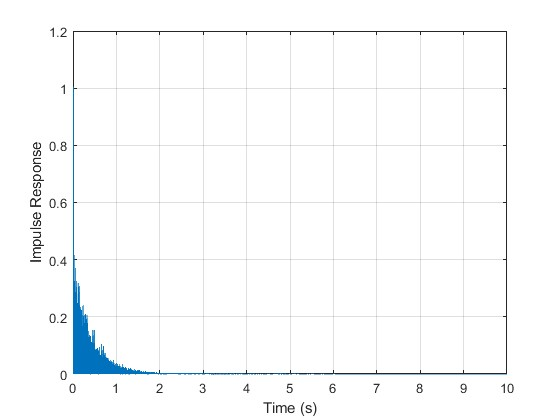
\includegraphics[width=\linewidth]{imagenes/RIRsquared_Simulated.jpg}
    \caption{\footnotesize RIR cuadrada obtenida de simulación}
    \label{fig:RIRsqSimulated}
\end{figure}
\FloatBarrier
A esta respuesta al impulso podemos aplicarle los mismos análisis que hacíamos con una respuesta al impulso obtenida mediante una medición.
\begin{figure}[!htb]
    \centering
    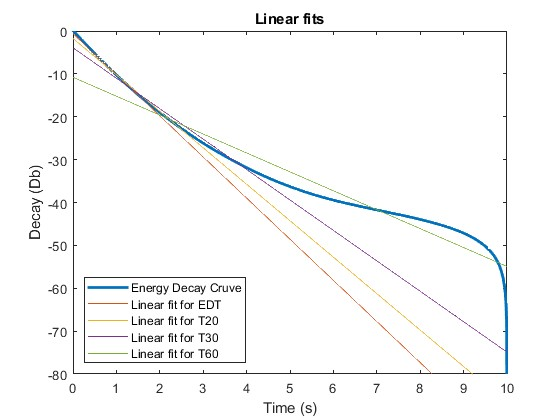
\includegraphics[width=\linewidth]{imagenes/RIRSimulated_Analysis.jpg}
    \caption{\footnotesize Análisis de la respuesta al impulso simulada}
    \label{fig:RIRSimulated_Analysis}
\end{figure}
\FloatBarrier
%------------------------------------------------------------------------------------------
Para comprobar el funcionamiento de nuestra simulación, recurrimos al uso de una paquetería de Python llamada PyRoomAcoustics, la cual permite hacer la simulación tal como la hicimos en MATLAB, pero de manera mas eficiente y con métodos mas completos. Sin profundizar en el funcionamiento, se creo un cuarto igual al de la implementación de MATLAB y se simulo la respuesta al impulso (Se adjunta el codigo utilizado en Anexo ?).
\begin{figure}[!htb]
    \centering
    \begin{subfigure}{0.3\textwidth}
        \centering
        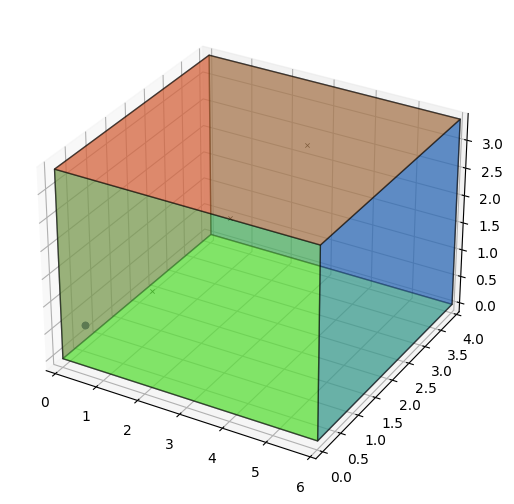
\includegraphics[width=\linewidth]{imagenes/PyRoom_Room.png}
        \caption{\footnotesize Cuarto simulado en PyRoomAcoustics}
        \label{fig:sub2_1}
    \end{subfigure}
    \hfill
    \begin{subfigure}{0.3\textwidth}
        \centering
        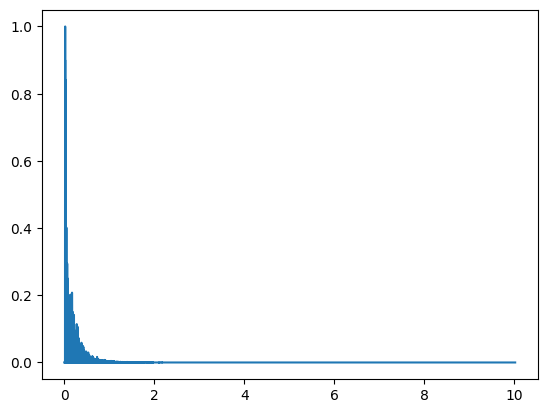
\includegraphics[width=\linewidth]{imagenes/PyRoom_RIR.png}
        \caption{\footnotesize Respuesta al impulso en PyRoomAcoustics}
        \label{fig:sub2_2}
    \end{subfigure}
    \hfill
    \begin{subfigure}{0.3\textwidth}
        \centering
        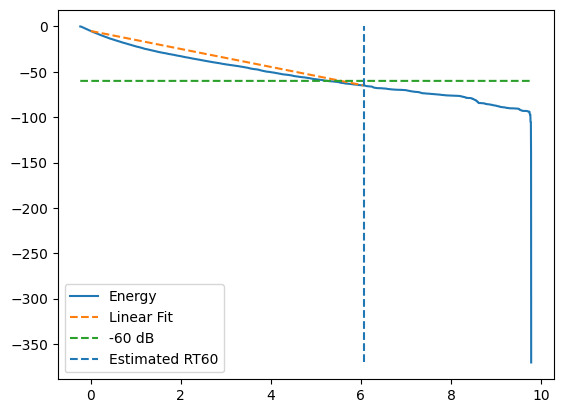
\includegraphics[width=\linewidth]{imagenes/PyRoom_Decay.png}
        \caption{\footnotesize Análisis de la respuesta al impulso en PyRoomAcoustics}
        \label{fig:sub2_3}
    \end{subfigure}
    \caption{Simulación con PyRoomAcoustics}
\end{figure}
\FloatBarrier
Como se puede observar, la simulación en Python arroja resultados muy similares a los obtenidos con la implementación en MATLAB. En el caso de MATLAB, el tiempo de reverberación calculado fue de $6.19 segundos$ mientras que en Python fue de $6.024 segundos$, un tiempo muy cercado considerando que se pierde resolución conforme aumenta el tiempo de reverberación debido a la naturaleza exponencial del decaimiento. \\
Una vez comprobada la implementación en MATLAB, podemos utilizarla con características localizadas de los materiales en las paredes. La simulación aun no es capaz de generar la respuesta al impulso de un recinto lleno (de instrumentos, muebles, decoración, etc.) debido a la complejidad de las interacciones. Para este propósito se buscara la utilización de un software especializado llamado CADNAR.

%-----------------------------------------------------------------------------------

\subsubsubsection{MF1.2 Procesamiento de la estrategia de control}

El control del sistema se hará mediante una ley de control de lazo cerrado de tipo PID. Se decidió hacer uso de esta estrategia básica debido a la transmisión de engrane de corona que tiene el sistema. \\
El sistema de transmisión permite un desacople de inercias, esto gracias a que en caso que el tornillo no se mueve, el eje perpendicular que contiene la corona no puede moverse por su propia inercia inercia, ya que sus dientes se detienen con los dientes del tornillo (que no cuentan con movimiento en el eje perpendicular al de la corona). Por lo anterior, se puede hacer el control del eje del tornillo tomando en cuenta para el control, únicamente la inercia y amortiguamiento efectivo de este. El peso del eje de la corona, se puede ver como una fuerza externa que se aplica sobre el sistema principal y que se sopesa mediante el control PID. \\
El propósito del control es hacer que el eje del prisma triangular, se mueva un tercio de vuelta por vez, y que permita que en cada tercio de vuelta, los solenoides puedan desacoplar los paneles que deben quedarse en esa posición. \\
Se hará uso de un control por trayectoria, con una interpolación con polinomios de Bezier, ya que nos permitirá un movimiento suave de aceleración y desaceleración del motor. \\
Los polinomio interpolador de grado $2n-1$ tiene la siguiente formula:

% \begin{dmath}
$\mu(t, t_1, t_2) = \mu(\delta) = \delta^{3}\left(\gamma_1 - \gamma_2\delta + \gamma_3\delta^{2} - \gamma_4\delta^{3} + \dots + \left(-1 \right)^{n-1}\gamma_n\delta^{n-1}  \right)$
% \end{dmath}

Donde $\delta$ es igual a $\frac{t - t_1}{t_2 - t_1}$ \\
En este caso utilizaremos un polinomio de grado 11, entonces $n = 6$.

% \begin{dmath}
$\mu(\delta) = \delta^{6}\left(\gamma_1 - \gamma_2\delta + \gamma_3\delta^{2} - \gamma_4\delta^{3}+ \gamma_5\delta^{4} - \gamma_6\delta^{5} \right)$
% \end{dmath}

Los polinomios cuentan con la condición de frontera, $\mu(1) = 1$, y por tanto, las múltiples derivadas, son iguales a cero. Se pueden utilizar estas condiciones de frontera para encontrar los parámetros $\gamma$, los cuales son únicos para un polinomio de cierto grado. En nuestro caso, las $\gamma$ son:
\begin{itemize}
    \item $\gamma_1 = 175.63$
    \item $\gamma_2 = 548.18$
    \item $\gamma_3 = 601.36$
    \item $\gamma_4 = 216.36$
    \item $\gamma_5 = -45.81$
    \item $\gamma_6 = -34.86$
\end{itemize}
Por ultimo, se puede escribir la interpolación completa como:
\[
    q = \left\{
    \begin{array}{ll}
        q_0 & t \leq t_0 \\
        q_0+(q_1-q_0)\mu(\delta) & t_0\leq t \leq t_1 \\
        q_1 & t \geq t_1
        \end{array}
        \right.
\]

%\[q = \begin{cases}
%    q_0 & t \leq t_0 \\
%    q_0 + \left(q_1-q_0 \right)\mu\left(\delta \right) & t_0 < t < t_1 \\
%    q_1 & t \geq t_1
%\end{cases}\]
Se pueden utilizar las ecuaciones para la posición y las primeras dos derivadas, la velocidad y aceleración, para pasar la trayectoria al controlador PID. \\
Se hizo la validación de la trayectoria por medio de Simulink. 
\begin{figure}[!htb]
    \centering
    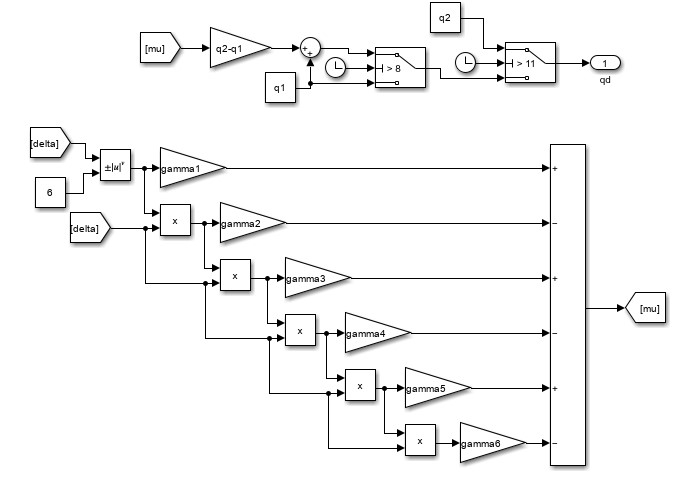
\includegraphics[width=1\textwidth]{imagenes/BezierIn.jpg}
    \caption{\footnotesize Interpolación de Bezier}
    \label{fig:BezierIn}
\end{figure}
\FloatBarrier
Es importante notar que esto hace una interpolación de una posición a otra, pero nuestra implementación requiere que se haga una interpolación de una posición a otra, esperar en esa posición y posteriormente hacer otra interpolación de esa posición a la siguiente. Debido a esto se utilizaran tres interpolaciones, las cuales se seleccionaran en función del tiempo transcurrido.
\begin{figure}[!htb]
    \centering
    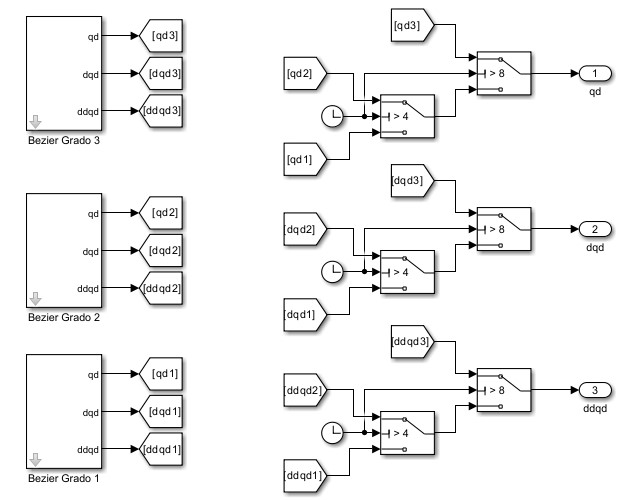
\includegraphics[width=1\textwidth]{imagenes/TripleInterpolationBezier.jpg}
    \caption{\footnotesize Triple Interpolación con polinomios de Bezier}
    \label{fig:TripleInterpolationBezier}
\end{figure}
\FloatBarrier
Los únicos parámetros que tomara entonces la interpolación de entre dos posiciones, sera el tiempo inicial y final de la interpolación, además de las posiciones iniciales y finales.
\begin{figure}[!htb]
    \centering
    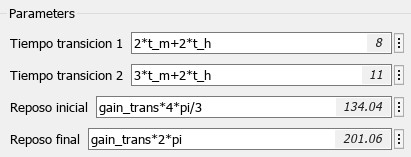
\includegraphics[width=0.6\textwidth]{imagenes/ParamsBezier.jpg}
    \caption{\footnotesize Parámetros de polinomio de Bezier}
    \label{fig:BezierParams}
\end{figure}
\FloatBarrier
Estos parámetros son fijos, y dependen de la implementación. En nuestro caso, ya que queremos que el eje de la corona de un tercio de vuelta en cada trayectoria, entonces las posiciones del eje del tornillo irán desde cero hasta $RT*n*2*pi/3$. Donde $RT$ es la ganancia debido a la transmisión de corona y $n$ va de 1 a 3, que son las posiciones que va a tomar. \\
Externamente, la interpolación triple solo tomara tres parámetros, el tiempo que le tomara al sistema realizar un tercio de vuelta, el tiempo que esperará para permitir el desacoplamiento de los paneles y la relación de transmisión de la transmisión de corona. \\
La ley de control de un PID es la siguiente:
% \begin{dmath}
$u = J\left(-k_p(q-q^{*})-k_i\int(q-q^{*})\partial t-k_d\left(\frac{\partial q}{\partial t}-\frac{\partial q^*}{\partial t}\right)\right)+B\frac{\partial q^*}{\partial t}+J\frac{\partial^2 q^*}{\partial t^2}$
% \end{dmath}
Donde $q$ es la posición y $dq$ y $ddq$, la velocidad y la aceleración respectivamente. La notación $q^*$ indica los parametros de la trayectoria.
Adicionalmente para la calibración de las ganancias debemos calcular los parámetros $\zeta$ y $\omega_n$, mediante las siguientes formulas:
% \begin{dmath}
$\zeta = \frac{log\left(\frac{Mp}{100}\right)}{\sqrt{\pi^{2}+\left(log\left(\frac{Mp}{100}\right) \right)^{2}}}$
% \end{dmath}
% \begin{dmath}
$\omega_n = \frac{3}{\zeta t_s}$
% \end{dmath}
Donde $t_s$ es el tiempo de asentamiento y $Mp$ es el máximo sobre impulso. \\
La ganancia integral se define estocásticamente, mientras que la ganancia derivativa se define como $k_d = 2\zeta\omega_n$ y la ganancia proporcional como $k_p = \omega_n^2$. \\
Los parámetros externos de la interpolación y del control PID se hicieron mediante mascaras para poder cambiar rápidamente los parámetros. \\
Para la validación del control de trayectorias, se usara el paquete de Simscape para simular la inercia y el amortiguamiento del tornillo sinfín. Se utilizara un fuente de torque ideal como el motor y un sensor rotacional para medir la posición y la velocidad del eje. 
\begin{figure}[!htb]
    \centering
    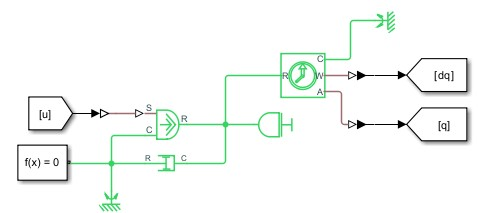
\includegraphics[width=1\textwidth]{imagenes/Simscape.jpg}
    \caption{\footnotesize Validación mediante Simscape}
    \label{fig:Simscape}
\end{figure}
\FloatBarrier
Por ultimo se hizo la simulación para comprobar el seguimiento del sistema de la trayectoria planeada.
\begin{figure}[!htb]
    \centering
    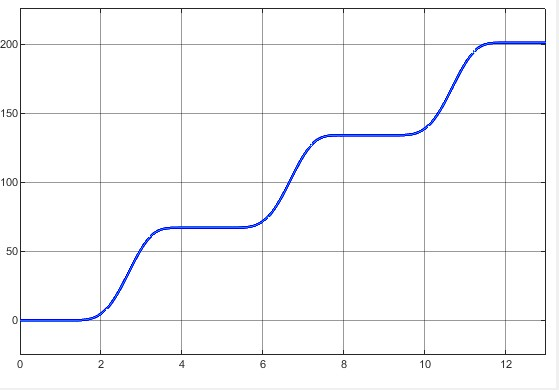
\includegraphics[width=1\textwidth]{imagenes/Trajectory.jpg}
    \caption{\footnotesize {Trayectoria y movimiento simulado}}
    \label{fig:Trajectory}
\end{figure}
\FloatBarrier
Se realizo un código que simularía la lógica detrás de los disparos de los solenoides para desacoplar cada panel al llegar a la posición deseada.\\ El código genera el vector de tiempo en función de los parámetros externos de la trayectoria para cada uno de los paneles y cuando se llega al tiempo de espera entre las trayectorias, el programa dispara los solenoides correspondientes a la posición en la que se encuentre (1,2,3). En el código, el vector \textit{arrange} contiene las posiciones de cada uno de los paneles, y \textit{Signals} es la matriz que contiene el estado en cada instante del tiempo de cada uno de los paneles.
\begin{lstlisting}[frame=single,numbers=left, style=Matlab-editor, basicstyle=\tiny]
for i = 1:num_panels
    if arrange(i) == 2
        Signals(i,offset1+((time_of_motion+time_of_hold)/step):end-1/step) = 1;
        offset1 = offset1 + 10;
    elseif arrange(i) == 3
        Signals(i,offset2+(2*time_of_motion+2*time_of_hold)/step:end-1/step) = 1;
        offset2 = offset2 + 10;
    elseif arrange(i) == 1
        Signals(i,offset3:end-1/step) = 1;
        offset3 = offset3 + 10;
    end   
end
\end{lstlisting}
Para ejemplificar el funcionamiento tomemos el vector \textit{arrange} como $[1,2,3,2,1,3]$. Al iniciar la simulación se dispararan inmediatamente los solenoides de los paneles 1 y 5, y permanecerán activados por el resto de la simulación. Cuando pasen $tiempo de movimiento + tiempo de espera$ segundos, el sistema ya habrá acabado el primer tercio de vuelta, en ese momento se activan los solenoides de los paneles 2 y 4. De igual manera, al haber pasado $2*tiempo de movimiento + 2*tiempo de espera$ segundos, el sistema habrá dado dos tercios de vuelta y activará los solenoides 3 y 6. Es importante notar que la trayectoria lleva a los paneles a la posición inicial (posición 1), y cuando ya se completó toda la vuelta, se desactivan todos los solenoides para llevar el sistema al estado de espera. Podemos ver una simulación de los disparos con las siguientes posiciones al lado de la trayectoria. $arrange = [1,2,2,3,3,1,2,1,3]$
\begin{figure}[!htb]
    \centering
    \begin{subfigure}{0.4\textwidth}
        \centering
        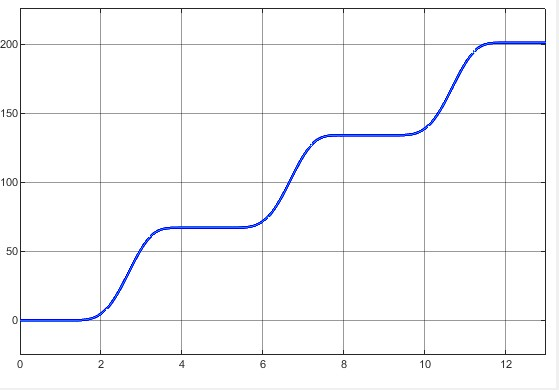
\includegraphics[width=\linewidth]{imagenes/Trajectory.jpg}
        \caption{\footnotesize Trayectoria simulada}
        \label{fig:Coils1}
    \end{subfigure}
    \hfill
    \begin{subfigure}{0.6\textwidth}
        \centering
        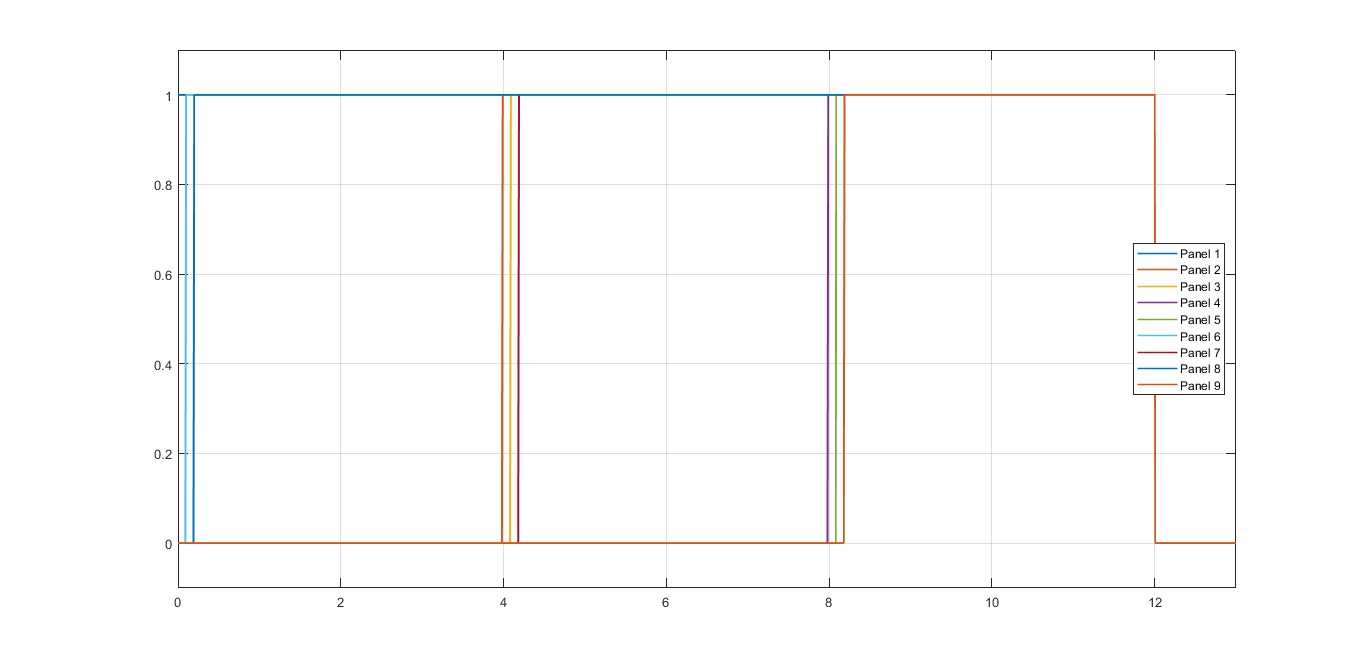
\includegraphics[width=\linewidth]{imagenes/AllCoilActivations.jpg}
        \caption{\footnotesize Activaciones de los solenoides}
        \label{fig:Coils2}
    \end{subfigure}
    \hfill
    \caption{Activación de los solenoides a lo largo de la trayectoria}
\end{figure}
\FloatBarrier

Se puede observar que al menos en la simulación, lo único que rige el movimiento del tornillo sinfín es la inercia y el amortiguamiento, y, debido a que el controlador toma en cuenta la inercia efectiva y el amortiguamiento efectivo para el calculo de la ley de control; el seguimiento presenta muy poco error. Además, al hacer un seguimiento de trayectoria en lugar de una referencia constante como en un impulso, se reduce en gran medida el sobre impulso y el tiempo de asentamiento. Se espera que en las pruebas físicas, se presente un error un poco mayor al previsto por la simulación debido al efecto de la masa del prisma triangular actuando como fuerza externa. \\

%------------------------------------------------------------------------

\subsubsubsection{MF1.3 Interacciones del sistema}

Este módulo se encarga de recibir las instrucciones de acondicionamiento emitidas por el usuario en la interfaz, así como de disponer la información necesaria para que pueda visualizarse en la interfaz, es donde los diferentes programas que componen al proyecto interactúan bajo la arquitectura descrita en la figura \ref{fig:ArquitecturaComunicacion}.\\

\begin{figure}[h]
    \centering
    \includegraphics[width=0.75\linewidth]{imagenes/ArquitecturaComunicación.png}
    \caption{Arquitectura de comunicación MF1.3}
    \label{fig:ArquitecturaComunicacion}
\end{figure}

\paragraph{Protocolo de comunicación}
%
La integración entre el dispositivo físico seleccionado para el procesamiento (Raspberry Pi) y el PC de escritorio propio del usuario, en el que vivirá el programa de interfaz de usuario, se comunica mediante el protocolo de transferencia de hipertexto (HTTP). Considerando la oferta de protocolos disponibles, y sus distintas ventajas y desventajas, se presenta a continuación una tabla \ref{tab:comparacion_protocolos} de comparación que destaca las características clave de otros protocolos relevantes. Esta tabla sirve como referencia para evaluar la idoneidad de HTTP en comparación con alternativas como MQTT, CoAP, WebSockets y gRPC, proporcionando una visión general de las opciones disponibles y ayudando a respaldar la elección final del protocolo HTTP en el contexto específico de este proyecto.\\
%
\begin{longtable}{|m{3cm}|m{6cm}|m{6cm}|}
\hline
\textbf{Protocolo} & \textbf{Ventajas} & \textbf{Desventajas} \\
\hline\raggedright
MQTT \cite{mqtt}\\(Message Queuing Telemetry Transport) & Es un protocolo ligero diseñado para conexiones remotas con dispositivos con recursos limitados y redes de ancho de banda restringido. Ideal para redes de sensores y aplicaciones de telemetría debido a su bajo consumo de datos. & Menor compatibilidad con aplicaciones web estándar. Requiere un broker MQTT adicional para gestionar la comunicación. \\
\hline\raggedright
CoAP \cite{coap}\\(Constrained Application Protocol) & Diseñado para dispositivos con recursos limitados en redes de baja potencia. Es similar a HTTP pero más ligero, utilizando UDP en lugar de TCP. & Menos soporte y herramientas en comparación con HTTP. No es tan ampliamente adoptado, lo que puede limitar la interoperabilidad. \\
\hline\raggedright
WebSockets \cite{websockets} & Permite comunicación bidireccional en tiempo real entre el cliente y el servidor. Es ideal para aplicaciones que requieren actualizaciones en tiempo real como chats y juegos en línea. & Puede ser más complejo de implementar y gestionar en comparación con HTTP. Requiere soporte tanto en el servidor como en el cliente para mantener la conexión activa. \\
\hline\raggedright
gRPC \cite{grpc}\\(gRPC Remote Procedure Calls) & Protocolo de alto rendimiento basado en HTTP/2 que permite la llamada a procedimientos remotos (RPC). Ideal para comunicaciones eficientes entre servicios. & Puede ser más complejo de implementar y requiere que ambos extremos (cliente y servidor) soporten gRPC. No es tan adecuado para aplicaciones con interfaces web estándar. \\
\hline
\caption{Comparación de protocolos de comunicación}
\label{tab:comparacion_protocolos}
\end{longtable}
%
La elección de HTTP como protocolo de comunicación en este proyecto se debe los siguientes criterios:
%
\begin{itemize}
    \item \textbf{Interoperabilidad}: HTTP es ampliamente compatible con servicios y aplicaciones web, lo que facilita la integración con otros sistemas y plataformas. Esto asegura que los diferentes componentes del sistema puedan comunicarse de manera efectiva sin problemas de compatibilidad.
    
    \item \textbf{Herramientas y Bibliotecas}: Existe una vasta cantidad de bibliotecas y herramientas disponibles para HTTP en Python, facilitando el desarrollo y la implementación. Esto permite a los desarrolladores aprovechar recursos existentes y reducir el tiempo de desarrollo.
    
    \item \textbf{Simplicidad y Conocimientos Previos}: HTTP es un protocolo conocido y ampliamente utilizado, lo que reduce la curva de aprendizaje y facilita la implementación y mantenimiento del sistema. Muchos desarrolladores ya están familiarizados con HTTP, lo que puede acelerar el proceso de desarrollo.
    
    \item \textbf{Seguridad y Escalabilidad}: HTTPS ofrece una capa de seguridad adicional mediante la encriptación de datos, protegiendo la información sensible durante la transmisión. Además, la integración con la nube proporciona escalabilidad y resiliencia, permitiendo que el sistema maneje un mayor volumen de datos y usuarios sin comprometer el rendimiento.
    
    \item \textbf{Ecosistema de Servicios}: Utilizar HTTP permite aprovechar una amplia gama de servicios en la nube y herramientas web. Esto incluye opciones para almacenamiento, procesamiento de datos y otros servicios que pueden integrarse fácilmente en el sistema, ofreciendo una solución completa y robusta.
\end{itemize}
%
Tras el análisis, en comparación con los distintos protocolos disponibles, se seleccionó HTTP debido a su amplio soporte, interoperabilidad con tecnologías web estándar y su capacidad para facilitar la transferencia de datos de manera segura y eficiente entre el procesador y el PC del usuario \cite{http}, lo que contribuye significativamente a la implementación exitosa de nuestro sistema con las tecnologías previamente seleccionadas que son MATLAB, Python, JavaScript y a la simbiótica integración que tienen estas con una arquitectura ampliamente utilizada en la industria como es el uso de la nube.
%
\paragraph{Nube}
La integración de un servidor en nube desempeña un papel fundamental en la infraestructura y el funcionamiento integral de nuestro proyecto. Debido a la naturaleza del mismo, tenemos que contar con recepción, análisis y transmisión de datos entre el dispositivo Raspberry Pi y el usuario final en su interfaz gráfica, estos servicios requieren de un entorno robusto y escalable que la nube puede proporcionar de manera efectiva, rápida y alcanzable para nuestro tiempo de desarrollo \cite{AnoteOnIoT}. \\

En primer lugar, la nube actúa como un repositorio centralizado para almacenar los datos generados en una base de datos. Esto garantiza la disponibilidad y la integridad de los datos, además de facilitar su acceso y gestión desde cualquier ubicación. La base de datos permite el almacenamiento estructurado y eficiente de la información relevante para el usuario. Otro aspecto crucial es la capacidad para ejecutar funciones y servicios de forma remota, lo que permite una interacción dinámica entre el usuario y el dispositivo Raspberry Pi. A través de esta infraestructura, el usuario puede enviar instrucciones y solicitudes que viajan por internet, y activan acciones específicas en el dispositivo, como puede ser una consulta de los últimos datos de lectura, o iniciar un nuevo acondicionamiento. \\

La utilización de la nube, es de ayuda para garantizar la escalabilidad, seguridad e interactividad necesarias para ofrecer una solución completa y eficiente a nuestras necesidades \cite{IoTandCloudConvergence}. La elección de un proveedor de nube adecuado se basa en los criterios de disponibilidad y confiabilidad en el servicio (uptime), ubicación del centro de datos, escalabilidad y flexibilidad, seguridad, servicios ofrecidos, costo. A continuación, se presenta una tabla de comparación \ref{tab:comparacion_nube1} entre diferentes ofertas de proveedores de servicios en la nube de acuerdo a estos criterios que nos ayudaron en la selección de nuestro proveedor.
%
\begin{longtable}{|m{4.5cm}|m{2.5cm}|m{5cm}|m{3cm}|}
\hline
\textbf{Proveedor de Nube} & \textbf{Uptime (\%)} & \textbf{Ubicación del Centro de Datos} & \textbf{Escalabilidad y Flexibilidad} \\
\hline
\textbf{Amazon AWS \cite{aws}} & 99.95 & Querétaro, México & Alta \\
\hline
\textbf{Google Cloud Platform GCP \cite{gcp}} & 99.95 & Los Angeles, US & Alta \\
\hline
\textbf{Microsoft Azure \cite{azure}} & 99.99 & Querétaro, México & Alta \\
\hline
\textbf{IBM Z Cloud \cite{ibmcloud}} & 99.95 & Dallas, US & Media-Alta \\
\hline
\textbf{Oracle Cloud \cite{oraclecloud}} & 99.95 & Querétaro, México & Media-Alta \\
\hline
\textbf{Digital Ocean \cite{digitalocean}} & 99.99 & San Francisco, US & Alta \\
\hline
\caption{Comparación de proveedores de nube según criterios}
\label{tab:comparacion_nube1}
\end{longtable}
%
Y una comparación entre la disponibilidad de servicios \ref{tab:comparacion_nube2}.
%
\begin{longtable}{|m{3.5cm}|m{1.5cm}|m{1.5cm}|m{1.5cm}|m{1.5cm}|m{1.5cm}|m{1.5cm}|}
\hline
\textbf{Servicio} & \textbf{AWS} & \textbf{GCP} & \textbf{Azure} & \textbf{IBM Cloud} & \textbf{Oracle Cloud} & \textbf{Digital Ocean} \\
\hline
\textbf{Almacenamiento} & \cellcolor{green!25}Sí & \cellcolor{green!25}Sí & \cellcolor{green!25}Sí & \cellcolor{green!25}Sí & \cellcolor{green!25}Sí & \cellcolor{green!25}Sí \\
\hline
\textbf{Computación} & \cellcolor{green!25}Sí & \cellcolor{green!25}Sí & \cellcolor{green!25}Sí & \cellcolor{green!25}Sí & \cellcolor{green!25}Sí & \cellcolor{green!25}Sí \\
\hline
\textbf{Red} & \cellcolor{green!25}Sí & \cellcolor{green!25}Sí & \cellcolor{green!25}Sí & \cellcolor{green!25}Sí & \cellcolor{green!25}Sí & \cellcolor{green!25}Sí \\
\hline
\textbf{Bases de Datos} & \cellcolor{green!25}Sí & \cellcolor{green!25}Sí & \cellcolor{green!25}Sí & \cellcolor{green!25}Sí & \cellcolor{green!25}Sí & \cellcolor{green!25}Sí \\
\hline
\textbf{IA/ML} & \cellcolor{green!25}Sí & \cellcolor{green!25}Sí & \cellcolor{green!25}Sí & \cellcolor{red!25}No & \cellcolor{red!25}No & \cellcolor{red!25}No \\
\hline
\caption{Comparación de proveedores de nube según servicios \cite{comparecloud}}
\label{tab:comparacion_nube2}
\end{longtable}
%
Entre los proveedores revisados, Google Cloud Platform (GCP) se destacó como la mejor opción por varias razones, ya que nos ofrece un uptime del 99.95, lo que garantiza una alta disponibilidad, además, contando con el hecho de que si bien no cuenta con el centro de datos más cercano actualmente, se anunció el lanzamiento de uno en Querétaro en un futuro próximo, por lo que la latencia, incluso con el actual en Los Angeles no representa un problema. Otro aspecto importante es el sólido soporte técnico que ofrece Google Cloud y su documentación clara. Es importante mencionar también que encontramos en este proveedor una amplia gama de servicios que si bien para los alcances actuales del proyecto solo requerimos de la computación, almacenamiento y bases de datos, permiten escalar las limitaciones actuales con herramientas de inteligencia artificial y machine learning, visión computacional, IoT, entre otros posibles servicios actualmente disponibles. Por último, en temas de costos, GCP nos facilita como estudiantes créditos para el desarrollo, y un costo por uso accesible para un futuro despliegue al ámbito productivo. En conjunto, todos estos aspectos hacen que Google Cloud Platform sea la opción más sólida y completa para satisfacer nuestras necesidades de infraestructura en la nube para este proyecto.\\

\paragraph{Base de datos}
%
Para la selección de la base de datos, consideramos principalmente la facilidad de acceso a los datos, y la flexibilidad sobre el tiempo, teniendo en cuenta que actualmente existen dos grandes opciones disponibles, SQL y noSQL, realizamos una comparación \ref{tab:comparacion_bd_sql_nosql} de las ventajas, desventajas y casos de uso documentados y utilizados actualmente en la industria para entender que opción se ajusta mejor a nuestro proyecto.\\
%
\begin{longtable}{|m{3cm}|m{5cm}|m{5cm}|}
\hline
\textbf{} & \textbf{SQL} & \textbf{NoSQL} \\
\hline
\textbf{Ventajas} & Estructura definida, transacciones ACID, escalabilidad vertical & Esquema flexible, escalabilidad horizontal, alto rendimiento \\
\hline
\textbf{Desventajas} & Esquema rígido, escalabilidad horizontal limitada, menor flexibilidad en datos no estructurados & Menor consistencia en algunos modelos, menor soporte para transacciones complejas, menor adopción en algunos casos \\
\hline
\textbf{Casos de Uso} & Aplicaciones con integridad de datos y transacciones seguras, proyectos con estructura de datos predefinida & Aplicaciones web escalables, manejo de datos no estructurados, análisis de big data \\
\hline
\caption{Comparación de Bases de Datos SQL y NoSQL \cite{SQLvsNoSQL}}
\label{tab:comparacion_bd_sql_nosql}
\end{longtable}
%
Con esto, rápidamente entendemos que el uso de una base de datos no relacional (noSQL) nos proporciona lo que buscamos, para entonces ahora definir el uso de alguno de los productos de esta categoría agregamos un criterio más, que es la integración con nuestro proveedor de nube.
Bajo esta condición seguimos encontrando una oferta amplia, desde bases de datos propias de Google hasta integraciones con terceros, entonces recurrimos a definir un último criterio de selección, que es el tipo de base de dato no relacional. En la siguiente tabla \ref{tab:comparacion_bases_datos} podemos encontrar una comparación entre las diferentes opciones, todas con integración para CGP.\\
%
\begin{longtable}{|m{2.2cm}|m{2.2cm}|m{6cm}|m{3cm}|}
\hline
\textbf{Base de Datos} & \textbf{Tipo} & \textbf{Descripción} & \textbf{Casos de uso}\\
\hline
\textbf
{Bigtable \cite{bigtable}} & 
Clave-valor &
Servicio de bases de datos NoSQL de alto rendimiento y totalmente gestionado, pensado para grandes cargas de trabajo analíticas y operativas. Procesa picos de más de 5000 millones de solicitudes por segundo y puede gestionar más de 10 exabytes de datos. &  
\begin{itemize}[label={}, leftmargin=0pt]
    \item Motores de recomendaciones
    \item Detección de fraudes
\end{itemize}\\
\hline
\textbf
{Firestore \cite{firestore}} & 
Documentos &
Servicio de bases de datos de documentos altamente escalable y muy popular, diseñado para el desarrollo móvil, web y de servidores, que permite hacer consultas más rápidas y fructíferas. & 
\begin{itemize}[label={}, leftmargin=0pt]
    \item Aplicaciones móviles, web y del Internet de las cosas
    \item Sincronización sin conexión
\end{itemize}\\
\hline
\textbf
{Memory store \cite{memorystore}} &
En memoria &
Acceso a los datos en un tiempo inferior a un milisegundo con Redis y Memcached totalmente gestionados. &
\begin{itemize}[label={}, leftmargin=0pt]
    \item Almacenamiento en caché
    \item Chats de redes sociales o feeds de noticias
\end{itemize}\\
\hline
\textbf
{MongoDB \cite{mongodb}} &
Documentos &
De código abierto que se destaca por su flexibilidad y escalabilidad. Su flexibilidad y capacidad para manejar datos no estructurados o semiestructurados lo hacen adecuado para proyectos donde la estructura de los datos puede cambiar con el tiempo o es difícil de modelar en un esquema relacional tradicional. &
\begin{itemize}[label={}, leftmargin=0pt]
    \item Aplicaciones móviles, web y del Internet de las cosas
    \item Gestión de contenido
\end{itemize}\\
\hline
\hline
\caption{Comparación de bases de datos compatibles con GCP y noSQL}
\label{tab:comparacion_bases_datos}
\end{longtable}
%
La decisión entre Firebase (Firestore) y MongoDB para el proyecto generó una discusión en torno a varios factores. Si bien ambas opciones son altamente escalables y populares en el desarrollo IoT, lo cual las hacen excelentes candidatas, MongoDB fue elegida como la mejor opción por las siguientes razones. En primer lugar, MongoDB tiene una mejor integración con Python, que es uno de los lenguajes de programación utilizados en el proyecto, esta estrecha integración facilita el desarrollo y la gestión de la base de datos dentro de nuestro entorno de trabajo. Además, MongoDB es una base de datos de código abierto, lo que nos da la confianza de uso por miles de usuarios en temas de seguridad y dirección de la tecnología a futuro. \\

\paragraph{Marco de trabajo para la conexión}

Es necesario un programa que haga la gestión de las funciones de cálculo y procesamiento, que realice las distintas operaciones en base de datos, y exponga los puntos de acceso para las solicitudes HTTP. Es decir, una pieza de software que integre las herramientas mencionadas hasta el momento en este módulo, este programa es conocido como el backend del proyecto \cite{backendDev}. \\
%
\begin{longtable}{|m{3cm}|m{3cm}|m{3cm}|m{3cm}|m{3cm}|}
\hline
\textbf{Características} & \textbf{Django \cite{django}} & \textbf{Flask \cite{flask}} & \textbf{FastAPI \cite{fastapi}} & \textbf{Spring Boot \cite{springboot}} \\
\hline
\textbf{Estructura y Modularidad} & Estructura completa, incluye ORM y autenticación & Microframework, altamente flexible & API-first, basado en OpenAPI & Framework completo, incluye muchas herramientas \\
\hline
\textbf{Facilidad de Gestión de CRUD} & Muy fácil, incluye un ORM potente & Necesita extensiones como SQLAlchemy & Rápido y sencillo con pydantic y SQLAlchemy & Incluye JPA y Hibernate para gestión de datos \\
\hline
\textbf{Integración con Servicios en la Nube} & Amplia integración con proveedores como AWS, GCP & Depende de extensiones y bibliotecas adicionales & Integración nativa con muchos servicios en la nube & Alta integración con servicios de nube empresarial \\
\hline
\textbf{Seguridad} & Incluye muchas características de seguridad por defecto & Depende del desarrollador implementar seguridad & Incluye características de seguridad, pero personalizables & Incluye muchas características de seguridad \\
\hline
\textbf{Escalabilidad} & Buena, adecuada para proyectos grandes & Mejor para proyectos pequeños a medianos & Alta escalabilidad gracias a su diseño asíncrono & Muy alta, adecuada para proyectos empresariales \\
\hline
\textbf{Velocidad de Desarrollo} & Rápido gracias a muchas herramientas integradas & Rápido para proyectos pequeños & Muy rápido para desarrollar APIs & Moderado, depende del tamaño del proyecto \\
\hline
\textbf{Documentación y Soporte} & Extensa documentación y gran comunidad & Buena documentación, comunidad activa & Buena documentación, creciendo en popularidad & Extensa documentación y soporte empresarial \\
\hline
\textbf{Comunidad y Ecosistema} & Muy grande, con muchas bibliotecas y herramientas & Grande, con muchas extensiones disponibles & Creciendo rápidamente, buena comunidad & Muy grande, con muchas herramientas empresariales \\
\hline
\textbf{Herramientas y Bibliotecas Predefinidas} & Incluye muchas bibliotecas útiles por defecto & Minimalista, depende de extensiones & Incluye herramientas para desarrollo rápido de APIs & Incluye muchas bibliotecas y herramientas \\
\hline
\caption{Comparación de Frameworks para Desarrollo Backend}
\label{tab:comparacion_backend}
\end{longtable}
%
En Python existen diversos marcos de trabajo con los cuales se puede desarrollar herramientas como esta, siendo Django nuestra mejor opción debido a su robustez y capacidad para manejar múltiples tareas de manera eficiente. Django ofrece una estructura clara y modular que facilita la gestión de la ejecución de códigos existentes, la realización de operaciones CRUD (crear, leer, actualizar, eliminar) en la base de datos, y esto viviendo desde la nube de GCP. Además, Django proporciona una gran cantidad de herramientas y bibliotecas predefinidas que simplifican la creación de endpoints (puntos de acceso) HTTP para la comunicación con la interfaz de usuario y la Raspberry Pi. Comparado con otras alternativas como Flask o FastAPI, Django destaca por su enfoque en la seguridad, la escalabilidad y la rápida velocidad de desarrollo, haciendo que sea una solución ideal para un proyecto que requiere una integración compleja y una gestión eficiente de recursos. \\